\section{Design and Implementation}

Throughout this section, we will detail the design decisions that led to the final implementation. 

\subsection{Initial Design}

First, we explain the initial design choices; detailing the functionalities of each component; i.e., the address incrementer, cache, decoder, ALUs and FSM; subsequently, we detail how these components interact with each other.

\subsubsection{Cache}

To store computation data, we make use of a 3$\times$88 word register matrix. Assuming that the images have a width of 352 byte sized pixels, 88 words store exactly one row ($352/4=88$).

The cache is organized into three horizontal register lines as follows:
\begin{itemize}
    \item the bottom line receives an incoming 32-bit word directly from the input buffer. When the fetch enable signal is asserted, the line selects the register corresponding to the fetch position signal (thanks to a 7-to-88 binary decoder), and stores such word into the selected register.
    \item The middle and top lines operate as parallel shift registers across the vertical axis. When the shift enabled signal is asserted, the entire bottom line is transferred to the middle, whereas the content of the middle line shifts to the top line.
\end{itemize}

\subsubsection{Address Incrementer}

The address incrementer is the component responsible for storing the address pointers.

\subsubsection{Sobel ALUs}

To compute the output word, the system makes use of 4 sobel ALUs

\subsubsection{Decoder}

In this initial architecture, the cache exposes all three full rows combinationally to the Pixel Decoder, allowing immediate access to any pixel neighborhood along the row without extra read latency.

\subsubsection{Finite State Machine}

The whole system is handled by a hybrid Mealy/Moore finite state machine (FSM); this module has the duty of managing all the other components in the accelerator. Initially, the FSM is supposed to be in the \texttt{IDLE} state. Once the \texttt{start} signal is asserted, the machine enters the \texttt{FETCH} state; here, it loads the first row of the image into the cache. Subsequently, the system enters the \texttt{SHIFT} state, which performs an upward shift in the cache; once the shift is completed, the fsm performs a series of 3 cycles (\texttt{WAIT\_0}, \texttt{WAIT\_1}, and \texttt{WAIT\_2}): 
\begin{itemize}
    \item the first asserts the \texttt{rd\_en} signal, requesting the next word from memory;
    \item the second inserts the received data into the cache (while asking for the second word);
    \item the third fetches the second word into cache.
\end{itemize}
Now the accelerator enters the \texttt{COMPUTE} state; where it computes one output word per cycle (four bytes at a time) and tells the address incrementer to advance read and write column indices; such process is repeated until the row ends. The accelerator must therefore pre-fetch two words before starting the computation since the last byte of the output word depends on the first byte of the second bottom word. Once the entire row has been computed (\texttt{wr\_row\_end=1}); the address incrementer moves the read and write pointers to the next row (\texttt{wr\_wrap=1} and \texttt{rd\_wrap=1}), and the cache performs an upward shift (by moving to \texttt{SHIFT}); the system then restarts from state \texttt{WAIT\_0}. This loop continues until the entire image has been filtered (\texttt{wr\_row\_end=1} and \texttt{wr\_col\_end=1}); here, \texttt{finish} is asserted, and the state machine goes back to \texttt{IDLE}.

\begin{figure}[H]
    \centering
\begin{tikzpicture}[
    >=Stealth,
    font=\sffamily,
    % --- State Node Styling ---
    every state/.style={
        rectangle,
        %draw=borderblue,
        %fill=fillblue,
        thick,
        minimum size=2.3cm,
        align=center,
        font=\ttfamily\bfseries\small,
        % drop shadow={shadow xshift=1.5pt, shadow yshift=-1.5pt, opacity=0.2}
    },
    % --- Transition Line Styling ---
    trans/.style={
        ->,
        >={Stealth[scale=1.1]},
        thick
    },
    % --- Label Badge Styling ---
    lbl/.style={
        font=\ttfamily\scriptsize,
        fill=white,
        draw=gray!30,
        thin,
        inner sep=3pt,
        rounded corners=2pt,
        align=center
    }
]

    % ==========================================================
    % NODE POSITIONS (Grid Layout)
    % ==========================================================
    
    % Top Row: Entry, Fetch, Shift
    \node[state, initial, initial text={\scriptsize rst\_n=0}, initial where=left] (IDLE) at (0, 0) {IDLE};
    
    \node[state] (FETCH) at (5.0, 0) {FETCH\\[2pt]\scriptsize rd\_inc=1};
    
    \node[state] (SHIFT) at (10.0, 0) {SHIFT\\[2pt]\scriptsize shift=1};

    % Bottom Row: Pipeline Delays & Compute
    \node[state] (WAIT0)   at (10.0, -5.0) {WAIT\_0\\[2pt]\scriptsize rd\_inc=1};
    
    \node[state] (WAIT1)   at (10.0, -10.0)  {WAIT\_1\\[2pt]\scriptsize rd\_inc=1};
    
    \node[state] (WAIT2)   at (5.0, -10.0)  {WAIT\_2\\[2pt]\scriptsize rd\_inc=1};
    
    \node[state] (COMPUTE) at (5.0, -5.0)  {COMPUTE\\[2pt]\scriptsize rd\_inc=1\\
                                                            \scriptsize wr\_inc=1};

    % ==========================================================
    % TRANSITIONS & MEALY OUTPUTS (Condition / Outputs)
    % ==========================================================
    \path[trans]
        % --- Top Row Transitions ---
        (IDLE)    edge[loop above] node[lbl] {start=0} (IDLE)
        (IDLE)    edge node[lbl] {start=1} (FETCH)
        
        (FETCH)   edge[loop above] node[lbl] {rd\_row\_end=0} (FETCH)
        (FETCH)   edge node[lbl] {rd\_row\_end=1 /\\ rd\_wrap=1} (SHIFT)

        % --- Shift -> Pipeline Chain ---
        (SHIFT) edge (WAIT0)

        % --- Pipeline Sequence (Right to Left) ---
        (WAIT0) edge (WAIT1)
        (WAIT1) edge (WAIT2)
        (WAIT2) edge (COMPUTE)

        % --- Compute Operations & Exit Loops ---
        (COMPUTE) edge[loop left] node[lbl] {wr\_row\_end=0} (COMPUTE)
        
        % Return to IDLE (Finished framing)
        (COMPUTE) edge node[lbl, pos=0.5] {wr\_row\_end=1 \& wr\_col\_end=1 /\\ 
                                        finish=1} (IDLE)
        
        % Curve back to SHIFT for next row
        (COMPUTE) edge node[lbl, pos=0.5] {wr\_row\_end=1 \& wr\_col\_end=0 /\\ wr\_wrap=1, rd\_wrap=1} (SHIFT);

\end{tikzpicture}
\caption{Finite State Machine Diagram}
\label{fig:fsm}
\end{figure}

\paragraph{Implementation Details.}

To maintain visual clarity in the state diagram (Figure~\ref{fig:fsm}), we omitted the output signals \texttt{rd\_en} and \texttt{wr\_en}. Such signals are derived combinationally: \texttt{wr\_en} directly mirrors the internal flag \texttt{wr\_inc}, asserting exclusively during the \texttt{COMPUTE} state; on the contrary, \texttt{rd\_en} is driven by \texttt{rd\_inc} across fetching, waiting, and compute states, but gated off during row boundaries or complete frame termination, that is
$$\texttt{rd\_en} = \texttt{rd\_inc} \;\wedge\; \neg(\texttt{rd\_row\_end} \;\vee\; \texttt{wr\_col\_end})$$

\begin{figure}[H]
\centering
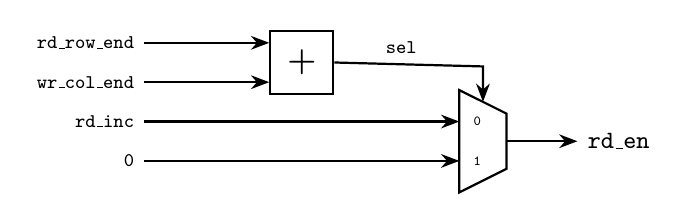
\begin{tikzpicture}[
    >=Stealth,
    font=\sffamily\small,
    thick
]

    % --- OR Gate ---
    \node[left, font=\ttfamily\scriptsize] (rd_row) at (0, 2.5) {rd\_row\_end};
    \node[left, font=\ttfamily\scriptsize] (wr_col) at (0, 2.0) {wr\_col\_end};

    \node[draw, rectangle, minimum size=0.8cm, font=\bfseries\large] (OR) at (2, 2.25) {+};

    % --- Data Inputs ---
    \node[left, font=\ttfamily\scriptsize] (rd_inc) at (0, 1.5) {rd\_inc};
    \node[left, font=\ttfamily\scriptsize] (zero)   at (0, 1.0) {0};

    % --- 2:1 MUX ---
    \draw (4.0, 0.6) -- (4.6, 0.9) -- (4.6, 1.6) -- (4.0, 1.9) -- cycle;
    \node at (4.5, 0.9) [font=\bfseries\scriptsize] {};
    
    % Internal Port Numbers (0 and 1)
    \node[font=\ttfamily\tiny, anchor=west] at (4.05, 1.5) {0};
    \node[font=\ttfamily\tiny, anchor=west] at (4.05, 1.0) {1};

    % --- Routing ---
    % OR Inputs
    \draw[->] (rd_row.east) -- (1.2, 2.5) |- (OR.west |- 0, 2.5);
    \draw[->] (wr_col.east) -- (1.2, 2.0) |- (OR.west |- 0, 2.0);

    % Select line from OR to top of MUX
    \draw[->] (OR.east) -- (4.3, 2.2) node[above, pos=0.45, font=\ttfamily\scriptsize] {sel} -- (4.3, 1.75);

    % MUX Data Inputs
    \draw[->] (rd_inc.east) -- (4.0, 1.5);
    \draw[->] (zero.east)   -- (4.0, 1.0);

    % MUX Output
    \draw[->] (4.6, 1.25) -- (5.5, 1.25) node[right, font=\ttfamily\bfseries\small] {rd\_en};

\end{tikzpicture}
\caption{Gated logic diagram for \texttt{rd\_en}.}
\label{fig:rd_en_mux}
\end{figure}

\subsection{System Structure}

Remember that fetch\_pos a and fetch\_en are delayed by one cycle through ffs

\tikzset{
  blk/.style={draw, thick, rounded corners=2pt, align=center},
  blk/.default=white,
  lab/.style={font=\ttfamily\scriptsize, inner sep=1.5pt},
  data/.style={-{Stealth[length=2.2mm]}, line width=1.3pt},
  ctrl/.style={-{Stealth[length=1.8mm]}, thick, black, dashed},
}
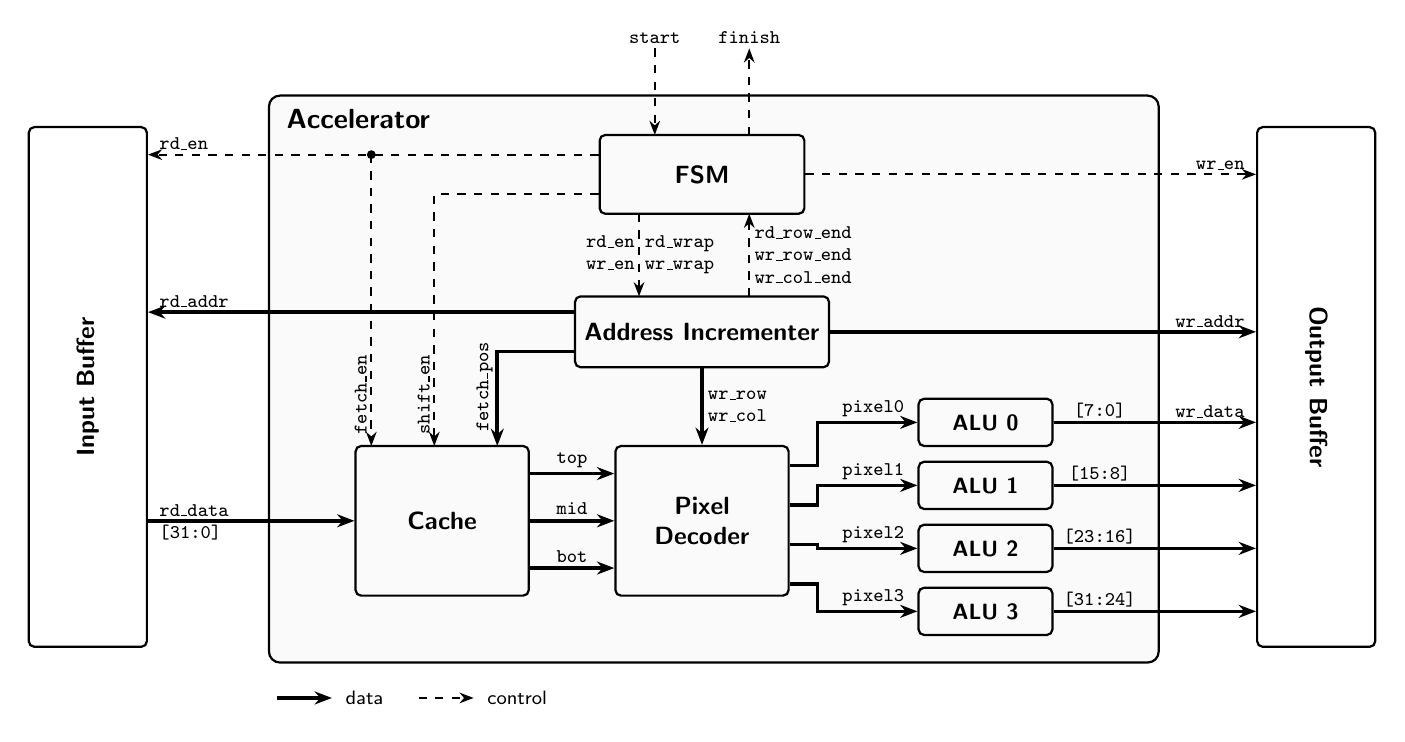
\begin{tikzpicture}[font=\sffamily\small]

  % ---------------- outer blocks ----------------
  \draw[thick, rounded corners=4pt, fill=gray!4] (2.3,0.1) rectangle (13.6,7.3);
  \node[anchor=north west, font=\sffamily\bfseries] at (2.4,7.25) {Accelerator};

  \node[blk, minimum width=1.5cm, minimum height=6.6cm] (ibuf) at (0.0,3.6)
       {\rotatebox{90}{\textbf{Input Buffer}}};
  \node[blk, minimum width=1.5cm, minimum height=6.6cm] (obuf) at (15.6,3.6)
       {\rotatebox{-90}{\textbf{Output Buffer}}};

  % ---------------- inner blocks ----------------
  \node[blk, minimum width=2.6cm, minimum height=1.0cm] (fsm)  at (7.8,6.3) {\textbf{FSM}};
  \node[blk, minimum width=3.0cm, minimum height=0.9cm] (addr) at (7.8,4.3) {\textbf{Address Incrementer}};
  \node[blk, minimum width=2.2cm, minimum height=1.9cm] (cache) at (4.5,1.9) {\textbf{Cache}};
  \node[blk, minimum width=2.2cm, minimum height=1.9cm] (dec)   at (7.8,1.9) {\textbf{Pixel}\\\textbf{Decoder}};
  \foreach \i/\y in {0/3.15,1/2.35,2/1.55,3/0.75}{
    \node[blk, minimum width=1.7cm, minimum height=0.6cm] (alu\i) at (11.4,\y) {\footnotesize \textbf{ALU \i}};
  }

  % ---------------- ibuf side ----------------
  \draw[ctrl] (fsm.west |- 0,6.55) -- (ibuf.east |- 0,6.55);
  \node[lab, anchor=south west] at (0.85,6.55) {rd\_en};
  \fill[black] (3.6,6.55) circle (1.6pt);
  \draw[ctrl] (3.6,6.55) -- (3.6,2.85);
  \node[lab, rotate=90, anchor=south] at (3.6,3.5) {fetch\_en};
  \draw[ctrl] (fsm.west |- 0,6.05) -- (4.4,6.05) -- (4.4,2.85);
  \node[lab, rotate=90, anchor=south] at (4.4,3.5) {shift\_en};
  \draw[data] (addr.west |- 0,4.55) -- (ibuf.east |- 0,4.55);
  \node[lab, anchor=south west] at (0.85,4.55) {rd\_addr};
  \draw[data] (addr.west |- 0,4.05) -- (5.2,4.05) -- (5.2,2.85);
  \node[lab, rotate=90, anchor=south] at (5.2,3.6) {fetch\_pos};
  \draw[data] (ibuf.east |- 0,1.9) -- (cache.west);
  \node[lab, anchor=south west] at (0.85,1.9) {rd\_data};
  \node[lab, anchor=north west] at (0.85,1.9) {[31:0]};

  % ---------------- cache -> decoder ----------------
  \draw[data] (cache.east |- 0,2.5) -- (dec.west |- 0,2.5) node[lab, above, midway] {top};
  \draw[data] (cache.east |- 0,1.9) -- (dec.west |- 0,1.9) node[lab, above, midway] {mid};
  \draw[data] (cache.east |- 0,1.3) -- (dec.west |- 0,1.3) node[lab, above, midway] {bot};

  % ---------------- FSM <-> addr_incrementer ----------------
  \draw[ctrl] (7.0,5.8) -- (7.0,4.75) node[lab, midway, xshift=4pt, align=right] {rd\_en rd\_wrap\\wr\_en wr\_wrap};
  \draw[ctrl] (8.4,4.75) -- (8.4,5.8) node[lab, midway, right, align=left] {rd\_row\_end\\wr\_row\_end\\wr\_col\_end};

  % ---------------- addr_incrementer -> decoder ----------------
  \draw[data] (addr.south) -- (dec.north) node[lab, midway, right, align=left] {wr\_row\\wr\_col};

  % ---------------- decoder -> ALUs ----------------
  \foreach \i/\y in {0/2.6,1/2.1,2/1.6,3/1.1}{
    \draw[data] (dec.east |- 0,\y) -- ++(0.35,0) |- (alu\i.west) node[lab, above, pos=0.78] {pixel\i};
  }

  % ---------------- obuf side ----------------
  \draw[ctrl] (fsm.east) -- (obuf.west |- fsm.east);
  \node[lab, anchor=south east] at (14.75,6.3) {wr\_en};
  \draw[data] (addr.east) -- (obuf.west |- addr.east);
  \node[lab, anchor=south east] at (14.75,4.3) {wr\_addr};
  \foreach \i in {0,1,2,3}{
    \draw[data] (alu\i.east) -- (obuf.west |- alu\i.east);
  }
  \node[lab, anchor=south] at (12.85,3.15) {[7:0]};
  \node[lab, anchor=south] at (12.85,2.35) {[15:8]};
  \node[lab, anchor=south] at (12.85,1.55) {[23:16]};
  \node[lab, anchor=south] at (12.85,0.75) {[31:24]};
  \node[lab, anchor=south east] at (14.75,3.15) {wr\_data};

  % ---------------- start / finish ----------------
  \draw[ctrl] (7.2,7.9) -- (7.2,6.8);
  \draw[ctrl] (8.4,6.8) -- (8.4,7.9);
  \node[lab, anchor=south] at (7.2,7.9) {start};
  \node[lab, anchor=south] at (8.4,7.9) {finish};
  \node[font=\sffamily\scriptsize, anchor=west, text=gray!40!black] at (9.0,8.0) {};

  % ---------------- legend ----------------
  \draw[data] (2.4,-0.35) -- ++(0.7,0);
  \node[anchor=west, font=\sffamily\scriptsize] at (3.15,-0.35) {data};
  \draw[ctrl] (4.2,-0.35) -- ++(0.7,0);
  \node[anchor=west, font=\sffamily\scriptsize] at (4.95,-0.35) {control};
  % \node[anchor=west, font=\sffamily\scriptsize, text=gray!40!black] at (6.4,-0.35)
       {in COMPUTE: 1 word read from ibuf and 1 word (4 output pixels) written to obuf per cycle};
\end{tikzpicture}

\subsection{Design Optimizations}

In the current state, the decoder is one of the most resource-intensive modules. The reason behind this stems from the immense number of inputs to this component, which corresponds to the size of the entire cache. The optimization we will implement, therefore, will aim at reducing the number of resources synthesized by developing a rotating cache design. Instead of scanning the cache linearly, this new system will only observe a fixed window, while the data will rotate in the opposite direction.

\subsubsection{Cache}

\subsubsection{Decoder}

The new decoder design simplifies the existing component: it does not receive the entire cache as input; on the contrary, it requires a small window of 6$\times$3 words. Such window corresponds to the first 5 columns of the cache plus the last as the further left one.

\usetikzlibrary{matrix, positioning, arrows.meta, calc, backgrounds, fit}

\begin{figure}[H]
    \centering
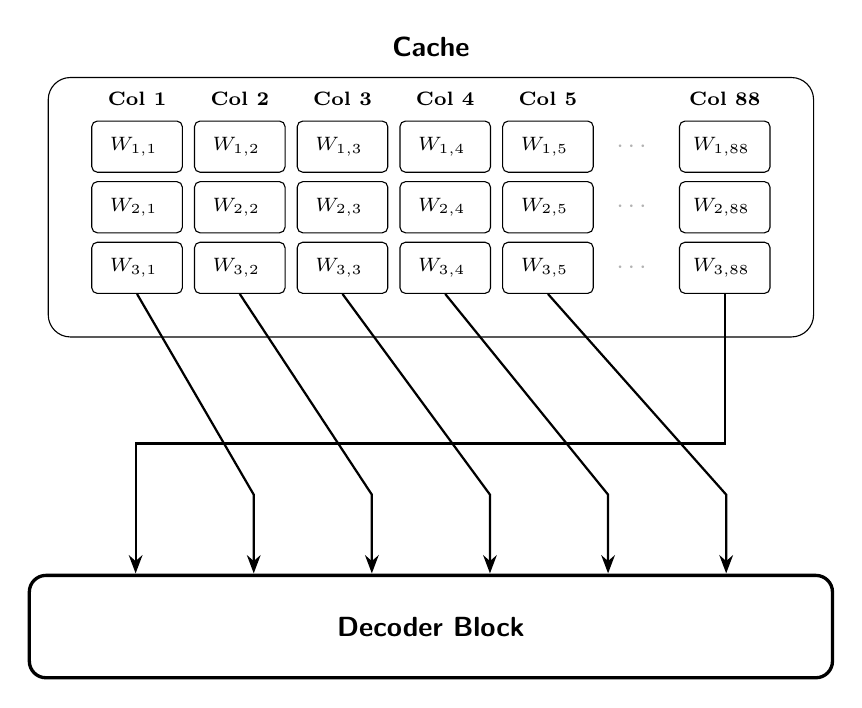
\begin{tikzpicture}[
    >=Stealth,
    font=\sffamily,
    % Cell definitions
    cell/.style={
        draw=black, 
        minimum width=1.15cm, 
        minimum height=0.65cm, 
        align=center, 
        font=\sffamily\scriptsize, 
        rounded corners=2pt
    },
    celllast/.style={
        draw=black, 
        minimum width=1.15cm, 
        minimum height=0.65cm, 
        align=center, 
        font=\sffamily\scriptsize\bfseries, 
        rounded corners=2pt
    },
    dots/.style={
        minimum width=0.8cm, 
        minimum height=0.65cm, 
        align=center, 
        font=\bfseries\small, 
        color=gray!60
    },
    % Block styles
    decoder/.style={
        draw=black, 
        rounded corners=6pt, 
        minimum width=10.2cm, 
        minimum height=1.3cm, 
        align=center, 
        font=\sffamily\bfseries, 
        line width=1.2pt
    },
    % Arrow styles
    arrow/.style={->, thick, black, >=Stealth},
]

% =============================================================
% TOP: 88x3 Words Cache
% =============================================================
\matrix (cache) [matrix of nodes, nodes={anchor=center}, column sep=4pt, row sep=3pt] {
    |[cell]| $W_{1,1}$ & |[cell]| $W_{1,2}$ & |[cell]| $W_{1,3}$ & |[cell]| $W_{1,4}$ & |[cell]| $W_{1,5}$ & |[dots]| $\cdots$ & |[celllast]| $W_{1,88}$ \\
    |[cell]| $W_{2,1}$ & |[cell]| $W_{2,2}$ & |[cell]| $W_{2,3}$ & |[cell]| $W_{2,4}$ & |[cell]| $W_{2,5}$ & |[dots]| $\cdots$ & |[celllast]| $W_{2,88}$ \\
    |[cell]| $W_{3,1}$ & |[cell]| $W_{3,2}$ & |[cell]| $W_{3,3}$ & |[cell]| $W_{3,4}$ & |[cell]| $W_{3,5}$ & |[dots]| $\cdots$ & |[celllast]| $W_{3,88}$ \\
};

% Cache column labels
\node[above=2pt of cache-1-1, font=\scriptsize\bfseries] {Col 1};
\node[above=2pt of cache-1-2, font=\scriptsize\bfseries] {Col 2};
\node[above=2pt of cache-1-3, font=\scriptsize\bfseries] {Col 3};
\node[above=2pt of cache-1-4, font=\scriptsize\bfseries] {Col 4};
\node[above=2pt of cache-1-5, font=\scriptsize\bfseries] {Col 5};
\node[above=2pt of cache-1-7, font=\scriptsize\bfseries] {Col 88};

% Cache container box
\begin{scope}[on background layer]
    \node[draw=black, rounded corners=8pt, fit=(cache) (cache-1-1) (cache-1-7), inner sep=12pt] (cache_box) {};
\end{scope}
\node[above=4pt of cache_box, font=\sffamily\bfseries] {Cache};

% =============================================================
% MIDDLE: Decoder Block
% =============================================================
\node[decoder, below=3cm of cache_box] (dec) {Decoder Block};

% 1) Last Column (Col 88 -> Leftmost slot in 6x3 window)

\draw[arrow] (cache-3-7.south) |- (0,-3.0) -| (-3.75,-4.65);
\draw[arrow] (cache-3-1.south) --(-2.25,-3.65) -- (-2.25,-4.65);
\draw[arrow] (cache-3-2.south) --(-0.75,-3.65) -- (-0.75,-4.65);
\draw[arrow] (cache-3-3.south) --(0.75,-3.65)  -- (0.75,-4.65);
\draw[arrow] (cache-3-4.south) --(2.25,-3.65)  -- (2.25,-4.65);
\draw[arrow] (cache-3-5.south) --(3.75,-3.65)  -- (3.75,-4.65);

% 2) First 5 Columns (Cols 1..5 -> Right 5 slots in 6x3 window)
\foreach \c [evaluate=\c as \targetcol using int(\c+1)] in {1,2,3,4,5} {
}

\end{tikzpicture}
    
    \caption{Cache to decoder window inputting.}
    \label{fig:placeholder}
\end{figure}


The module still performs boundary checks based on the current column and row indices, avoiding invalid inputs to the four Sobel ALUs. 

\subsection{FSM}

The new FSM design must output both the horizontal cache shift (\texttt{xshift}) and the cache fetch position (\texttt{fetch}). During the \texttt{FETCH} state, the accelerator fetches the input word into slot 0 of the cache and performs a horizontal shift (\texttt{fetch\_int=01, xshift=1}). After the \texttt{FETCH} state, a new state occurs (the \texttt{ALIGN} state); here, one cycle is used to perform a final horizontal rotation of the cache, needed to align the first word of the row with the first word of the cache. % WHY THIS HAPPENS 
The following state flow remains unchanged; whereas, the state outputs are modified as follows. \texttt{WAIT\_0} asserts \texttt{fetch\_int} to 01, while \texttt{WAIT\_1} and \texttt{WAIT\_2} assert \texttt{fetch\_int} to 10; finally, \texttt{COMPUTE} keeps fetching words from slot 1 of the cache (\texttt{fetch\_int=10}) while, at the same time, shifting the cache data horizontally.

\begin{figure}[H]
    \centering
\begin{tikzpicture}[
    >=Stealth,
    font=\sffamily,
    % --- State Node Styling ---
    every state/.style={
        rectangle,
        %draw=borderblue,
        %fill=fillblue,
        thick,
        minimum size=2.3cm,
        align=center,
        font=\ttfamily\bfseries\small,
        % drop shadow={shadow xshift=1.5pt, shadow yshift=-1.5pt, opacity=0.2}
    },
    % --- Transition Line Styling ---
    trans/.style={
        ->,
        >={Stealth[scale=1.1]},
        thick
    },
    % --- Label Badge Styling ---
    lbl/.style={
        font=\ttfamily\scriptsize,
        fill=white,
        draw=gray!30,
        thin,
        inner sep=3pt,
        rounded corners=2pt,
        align=center
    }
]

    % ==========================================================
    % NODE POSITIONS (Grid Layout)
    % ==========================================================
    
    % Top Row: Entry, Fetch, Shift
    \node[state, initial, initial text={\scriptsize \texttt{rst\_n=0}}, initial where=left] (IDLE) at (0, 0) {IDLE};
    
    \node[state] (FETCH) at (5.0, 0) {FETCH\\[2pt]  \scriptsize rd\_inc=1\\
                                                    \scriptsize fetch\_int=01\\
                                                    \scriptsize xshift=1};
    
    \node[state] (ALIGN) at (10.0, 0) {ALIGN\\[2pt]\scriptsize xshift=1};

    % Bottom Row: Pipeline Delays & Compute
    \node[state] (SHIFT)   at (10.0, -5.0) {SHIFT\\[2pt]\scriptsize yshift=1};
    
    \node[state] (WAIT0)   at (10.0, -10.0) {WAIT\_0\\[2pt] \scriptsize rd\_inc=1\\
                                                            \scriptsize fetch\_int=01};
    \node[state] (WAIT1)   at (5.0, -10.0)  {WAIT\_1\\[2pt] \scriptsize rd\_inc=1\\ 
                                                            \scriptsize fetch\_int=10};
    
    \node[state] (WAIT2)   at (0.0, -10.0)  {WAIT\_2\\[2pt] \scriptsize rd\_inc=1\\
                                                            \scriptsize fetch\_int=10};
    
    \node[state] (COMPUTE) at (0.0, -5.0)  {COMPUTE\\[2pt]  \scriptsize rd\_inc=1\\
                                                            \scriptsize wr\_inc=1\\
                                                            \scriptsize fetch\_int=10 \\
                                                            \scriptsize xshift=1};

    % ==========================================================
    % TRANSITIONS & MEALY OUTPUTS (Condition / Outputs)
    % ==========================================================
    \path[trans]
        % --- Top Row Transitions ---
        (IDLE)    edge[loop above] node[lbl] {start=0} (IDLE)
        (IDLE)    edge node[lbl] {start=1} (FETCH)
        
        (FETCH)   edge[loop above] node[lbl] {rd\_row\_end=0} (FETCH)
        (FETCH)   edge node[lbl] {rd\_row\_end=1 /\\ rd\_wrap=1} (ALIGN)

        % --- Shift -> Pipeline Chain ---
        (ALIGN) edge (SHIFT)
        (SHIFT) edge (WAIT0)

        % --- Pipeline Sequence (Right to Left) ---
        (WAIT0) edge (WAIT1)
        (WAIT1) edge (WAIT2)
        (WAIT2) edge (COMPUTE)

        % --- Compute Operations & Exit Loops ---
        (COMPUTE) edge[loop left] node[lbl] {wr\_row\_end=0} (COMPUTE)
        
        % Return to IDLE (Finished framing)
        (COMPUTE) edge node[lbl, pos=0.5] {wr\_row\_end=1 \& wr\_col\_end=1 /\\ 
                                        finish=1} (IDLE)
        
        % Curve back to SHIFT for next row
        (COMPUTE) edge node[lbl, pos=0.5] {wr\_row\_end=1 \& wr\_col\_end=0 /\\ wr\_wrap=1, rd\_wrap=1} (SHIFT);

\end{tikzpicture}
\caption{Modified Finite State Machine Diagram}
\label{fig:mod_fsm}
\end{figure}

This new design internally handles the "off by one cycle" delay and the boundary conditions of the cache fetching mechanism. That is, the output signal \texttt{fetch} is the sequential result of the \texttt{fetch\_int} signal, gated off with \texttt{rd\_en}. 
$$\texttt{fetch}=\texttt{fetch\_int}\cdot\texttt{rd\_en}$$